%\subsection{Goals}
\subsection{Access semantics and optimization goals}
\sys\ is a persistent ordered key-value store. Similarly to popular industrial ones~\cite{hbase,leveldb,RocksDB}, 
 it supports concurrent access by multiple threads and ensures 
strong consistency. 
%\begin{enumerate}\itemsep0pt
%\item 
Specifically its \emph{put, get}, and \emph{range scan} (or scan) operations are \emph{atomic}.  
For scans, this means that all key-value pairs returned by a single scan belong to a consistent 
snapshot reflecting the state of the data store at a unique point in time.

Additionally, \sys\ ensures {consistent recovery}: following a crash, the system recovers to a well-defined execution 
point.  
When persistence is \emph{asynchronous}, puts are buffered and persisted to disk in the background,  
 trading durability for speed. In this case, some recent updates may be lost but 
 recovery is to a \emph{consistent} state  
in the sense that if some put is lost, then no ensuing (and thus possibly dependent) puts are reflected in the data store.
%\end{enumerate}

Our key optimization goals are the following:
\begin{enumerate}
%\itemsep0pt
\item {\bf Optimize for spatial locality}, e.g., workloads that employ composite keys.
\remove{
 Many NoSQL applications embed multi-dimensional data in a single-dimension composite key. 
 This design provides high spatial locality on the primary dimension (key prefix). We strive
 to express this locality in physical data organization.
 }
 % to exploit it efficiently for scans  by the primary dimension. 
%In addition, a query that retrieves data pertaining to a particular dimension thus needs to atomically 
%retrieve the values pertaining to a range of keys. 
%To favor analytics queries, it is important to optimize such scans. 


\item {\bf Low write amplification}  to boost performance 
and reduce disk wear.%, especially for SSD devices.
 
\item {\bf High performance  with memory-resident working sets.}
%To sustain high speed, key-value stores nowadays leverage increasing RAM sizes where they can hold most of the active working set. 
We strive for high performance in the ``hyper-local'' scenario when most of the active working set fits in RAM. 
Note that we do \emph{not} expect the entire database to fit in
memory, only the active data.  
 
\item {\bf Fast consistent recovery.}  Because crashes are inevitable, recovery must ensure consistency and 
the downtime it entails should be kept  short. 
\end{enumerate}

\subsection{Design choices}

%We discuss our design choices and compare them to alternative KV-store designs.

% Given the aforementioned requirements, we make the following design choices:

%\paragraph{Data organization and caching.}

\sys\ combines the spatial locality of B-trees with the optimized I/O and quick access of LSM. 
Its data layout is illustrated in Figure~\ref{fig:piwi}.  We now discuss our key design choices.   

\begin{figure}[tb]
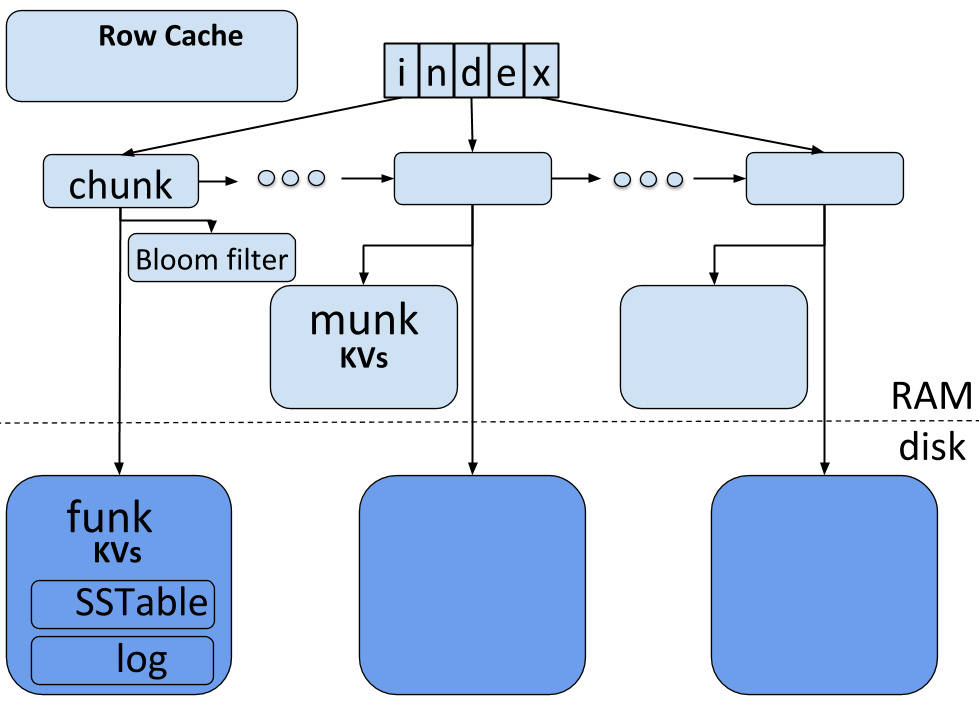
\includegraphics[width=\columnwidth]{PiWi.png}
\caption{\sys's  organization. Gray boxes depict metadata, light blue areas show RAM caches of KV-pairs, and blue areas represent on-disk KV storage.}
\label{fig:piwi}
\end{figure}


{\bf Spatial organization.\ }
In order to leverage spatial locality, we partition data -- both into files and in memory -- by key.
Our in-memory data structure is organized as a sorted linked list of \emph{chunks} holding consecutive key ranges.
The chunks themselves are lightweight metadata objects. They are volatile and are reconstructed from disk on recovery.

{\bf Sequential I/O with in-chunk logging.\ }
For persistence, each chunk has a file representation called  \emph{funk} (file chunk), which holds all the KV-pairs in the chunk's range.
Within funks, we adopt LSM's sequential I/O approach. To this end, the funk 
is divided into two parts: (1) a sorted \emph{SSTable} (Sorted String Table~\cite{Bigtable2008}), and (2) an unsorted \emph{log}. 
New updates are appended to the log; the log is  merged into the SSTable via an infrequent background compaction process. 
Unlike LSMs, \sys\ logs writes exclusively within their funks and avoids duplicating the updates  in a separate WAL. This reduces write amplification and expedites recovery. 

{\bf Key-range caching with in-memory compaction.\ }
Caching KV-pairs in RAM is instrumental for achieving high read performance in persistent KV-stores. 
Because we target workloads with high spatial locality, we employ caching at the granularity of chunks.
Namely, popular chunks are cached in a  memory data structure called \emph{munk} (memory chunk).
While traditionally, caching  only serves the read-path, working at the chunk granularity allows us to 
leverage it also in the write-path, specifically, for in-memory compaction.  Whereas appending writes to 
the log is essential for persistence, compacting the log is only required for performance (specifically, to 
reduce on-disk search time). But the latter is not required when the chunk is cached. Thus, when 
a chunk has a munk, we compact it almost exclusively in memory. 
%Note that typically only ``cold'' chunks do not have munks, and since little data is 

%\paragraph{Chunk-based organization for spatial locality}


% This organization exploits spatial locality and is friendly to range scans.




\remove{
\begin{figure*}[tb]
%\centerline{
\begin{subfigure}{0.34\linewidth}
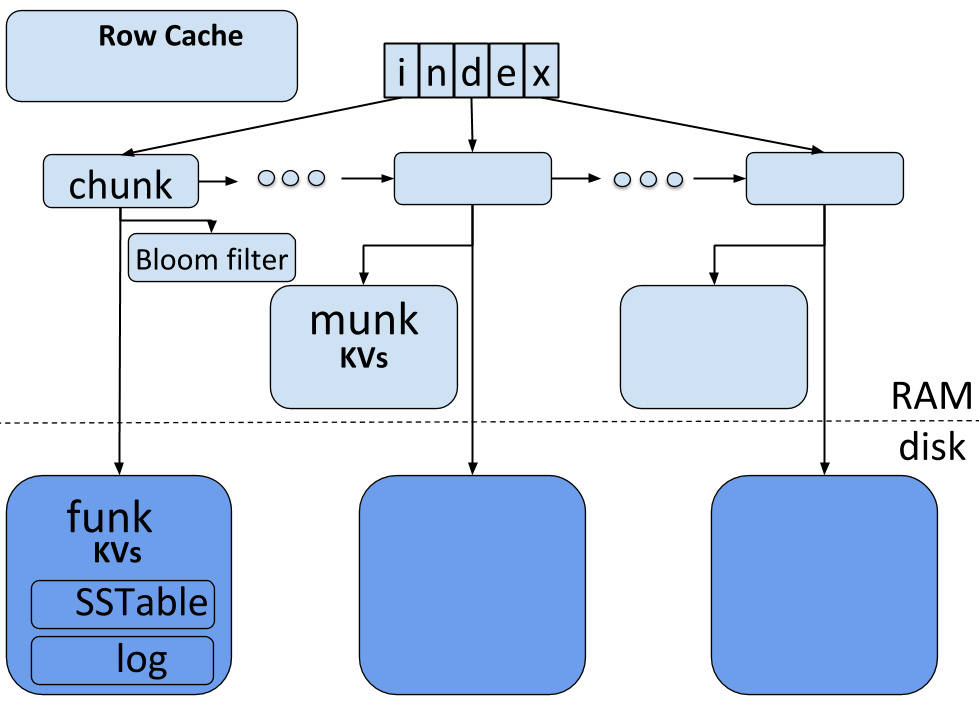
\includegraphics[width=\columnwidth]{PiWi.png}
\caption{\sys: data partitioned by key}
\label{fig:piwi}
\end{subfigure}
\hspace{1mm}
\begin{subfigure}{0.3\linewidth}
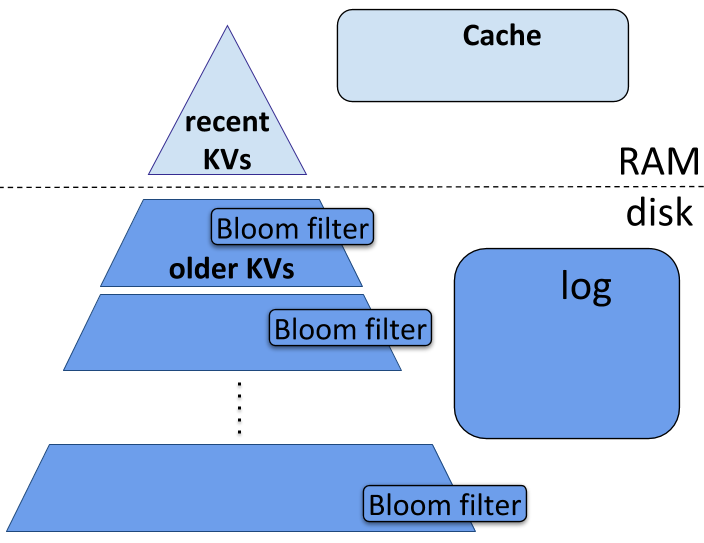
\includegraphics[width=\textwidth]{LSM.png}
\caption{LSM: temporal partitioning}
\label{fig:lsm}
\end{subfigure}
\hspace{1mm}
\begin{subfigure}{0.3\linewidth}
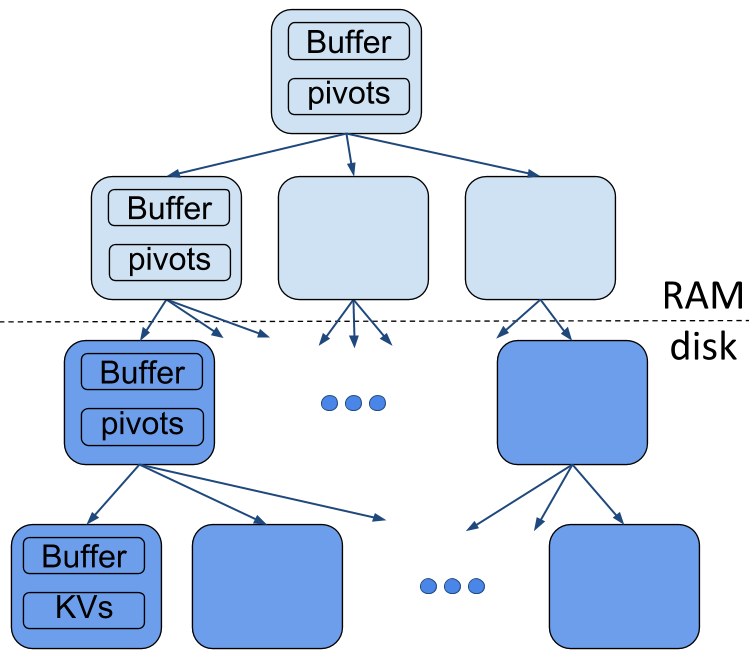
\includegraphics[width=\textwidth]{Bepsilon.png}
\caption{B$^\epsilon$  tree: data partitioned by key}
\label{fig:bepsilon}
\end{subfigure}
%}
\caption{\sys's data layout compared to LSMs and B$^\epsilon$ trees.}
\label{fig:layout}
\end{figure*}
}

Chunks are organized in a sorted linked list. To speed up key access, they are 
indexed using a volatile index (a sorted array in our implementation).  
We also partially sort the keys in each chunk for fast in-chunk search.  
 To expedite access to  keys whose chunks are only on-disk  (i.e., have no munks), 
individual popular keys are cached in a \emph{row cache}, 
and \emph{Bloom filters} are used to limit excessive access to disk. 

For comparison, an LSM tree (Figure~\ref{fig:lsm}), organizes data temporally, keeping only the most recent updates in memory.
The in-memory (top level) store optimizes the write-path. To optimize the read path, it uses a large cache.   
For persistence, data is logged to a WAL (write-ahead log). 

Another related data organization is that of  B-trees and B$^\epsilon$-trees (Figure~\ref{fig:bepsilon}), which also partition data by key range. 
B$^\epsilon$-trees use in-node update buffers, which resemble \sys's in-funk WALs.
However, their buffers are not used for persistence --- their intent is to amortize the $O(\log n)$ tree traversal cost across multiple updates. 
\remove{
These trees are analyzed in a model with no memory hierarchy, where all nodes are disk-resident. In practice, their upper layers 
are typically cached in RAM. Given such caching, amortizing the $O(\log n)$ traversal cost is not important, and indeed, practical data stores inspired by
such trees forgo the buffers in internal nodes. Thus, every write entails an in-place update of a leaf node, and every read requires disk access unless the node it reads is cached.
}

 %\emph{In-funk logs and infrequent disk compaction.}
\sys\ logs writes within funks and avoids duplicating the updates  in a separate WAL. This reduces write amplification and expedites recovery. 
The  log is merged into the chunk's sorted key-value table (\emph{SSTable} -- Sorted String Table~\cite{Bigtable2008}) 
via an infrequent background compaction process. 
While a chunk is cached (has a munk), there is no urgency to improve its on-disk organization since 
queries do not access it. Therefore, \sys\ infrequently performs reorganization (compaction) on such funks,
and compacts them only in-memory.
Conversely, when a funk holds cold data, its organization hardly deteriorates, so no compaction is needed.
Note that this is unlike LSM trees, where all disk components are compacted, regardless of which keys reside in memory.
% and whether keys are hot or cold. 


 \paragraph{Concurrency and multi-versioning.}
 \sys\ allows high parallelism among threads invoking its API calls. 
 Read operations are wait-free (never block) and puts use lightweight synchronization. 
 To support atomic scans, we  employ a light form of multi-versioning that uses 
copy-on-write to keep old versions only if they may be required by ongoing scans. 
In other words, if a put attempts to overwrite a key required by an active scan, then a new version is created alongside the 
existing one, whereas versions that are not needed by any scan are not retained. 
Thus, version management incurs a low overhead (as it occurs only on scans). 
%It also defines a simple rule for garbage collecting old versions.
In addition, tagging each value with a version allows \sys\ to easily recover to a consistent point in time, namely a version below which all puts have been persisted to disk.

To support atomic scans, production LSM stores employ standard MVCC on top of the LSM tree.  
Each write operation is assigned an auto-incremented sequence number. Since each write adds an additional version to the key it writes to, the memory component often overflows  even if the working set is small enough to fit in memory. This causes frequent data compactions and increases write amplification.
%Like in B-trees 


%Since updates are buffered in-memory in different paths of the tree before they are persisted in the leaves, supporting consistent recovery in multi-threaded workloads is also not trivial.

